\input{confgTex.tex}

%----------------------------------------------------------------------------------------
%	TÍTULO Y DATOS DEL ALUMNO
%----------------------------------------------------------------------------------------

\title{	
\normalfont \normalsize 
\textsc{\textbf{Prácticas de Empresa (2017-2018)} \\ Grado en Ingeniería Informática \\ Universidad de Granada} \\ [25pt] % Your university, school and/or department name(s)
\horrule{0.5pt} \\[0.4cm] % Thin top horizontal rule
\huge Memoria de Prácticas realizadas en EXPOELVIRA S.L. \\ % The assignment title
\horrule{2pt} \\[0.5cm] % Thick bottom horizontal rule
\begin{figure}[H] %con el [H] le obligamos a situar aquí la figura
	\centering
	\includegraphics[scale=0.5]{image/ugr.png}  %el parámetro scale permite agrandar o achicar la imagen. En el nombre de archivo puede especificar directorios
\end{figure}
}

\author{Antonio Rodríguez Alaminos} % Nombre y apellidos

\date{\normalsize\today} % Incluye la fecha actual

%----------------------------------------------------------------------------------------
% DOCUMENTO
%----------------------------------------------------------------------------------------

\begin{document}
	\maketitle
	
	\newpage
	\tableofcontents
	\newpage
	
	\part{Introducción}		\setcounter{section}{0}
	
		Este documento engloba la memoria de prácticas realizadas en la empresa \textit{\textbf{DEVENTOS} (EXPOELVIRA S.L.)}, entre marzo del 2018 y junio del 2018.\\
		
		Dicha empresa, dadas sus necesidades, nos ofreció un contrato a dos estudiantes del Grado en Ingeniería Informática; permitiéndonos trabajar en grupo y de forma autónoma, además de aprender y coger experiencia en diferentes sectores de la informática relacionados con los sistemas web, bases de datos, etc... satisfaciendo las distintas tareas necesarias para el desarrollo de dichas prácticas.\newline
		
		La duración de dicho contrato fue de 300 horas (es decir, 5 horas diarias de lunes a viernes, con horario totalmente flexible a nuestra disponibilidad, por condición de estudiantes y pudiendo trabajar desde casa). 
		
		\newpage
	
	\part{Descripción de la entidad donde realizó las prácticas}	\setcounter{section}{0}
	
		\section{Actividad laboral a la que se dedica la entidad}
		Deventos es una empresa pequeña situada en el polígono de Asegra en Granada, que desarrolla y comercializa el desarrollo de eventos. Esta, genera desde cero los eventos, alquilando desde el local hasta los stand, que luego compondrán el mismo evento.\newline
		
		Además, para actualizar la empresa a las nuevas tecnologías nuestra parte es formar un equipo capaz de dar servicio web, app-móvil y diversos servicio TIC para el desarrollo de los eventos. \\
		
		\begin{center}
			\includegraphics[scale=0.45]{image/asegra.jpg}\\
			Evento desarrollado por DEVENTOS - \href{https://www.facebook.com/encuentrojuncarilasegra/}{Faccebook}
		\end{center}
		
		\newpage
		
		\section{Personal cualificado tecnológicamente de que dispone}
		Como decíamos antes, se trata de una empresa pequeña que dispone de pocos empleados. Entre ellos, encontramos a dos diseñadores gráficos, a un dani(especialización dani), también tenemos un técnico de sonido e imagen para el desarrollo de los servicios multimedia de la empresa, y a diversos especialistas en montajes de mobiliario para dichos eventos (que forman parte del equipo, aunque no tengan parte del desarrollo de nuestro trabajo). \\ 
		
		Los estudiantes que nos incorporemos a realizar prácticas junto con los compañeros mencionados anteriormente, formamos toda la plantilla de informáticos que hay trabajando allí, por lo que no teniendo nadie con mas experiencia que nosotros, en el campo de desarrollo web, pudimos poner en práctica tareas de auto-gestión y hemos tenido que enfrentarnos a los problemas generados de forma autónoma. 
		
		\section{Dotación tecnológica de la que dispone}
		Dado el volumen actual de la empresa, se sitúan en un local mediano con el espacio suficiente para el desarrollo y montaje de dichos eventos. Cada uno de los ya empleados en la compañía utilizaban un equipo concedido por la empresa, pero cada estudiante trabajaba con su propio equipo portátil.\newline
		
		Además, del alquiler de un servidor que comentaremos posteriormente para el alojamiento del proyecto desarrollado, y diversas plantillas y software.\\
		
		En cuanto a conectividad y comunicación, la empresa dispone de conexión de fibra óptica de alta velocidad, por lo que cualquier labor que necesite conexión se hace mucho más cómoda y rápida.
		
		\newpage
		
	\part{Trabajo realizado}	\setcounter{section}{0}
		
		\section{Problemas que se han planteado}
		
		Al principio del período contractual se nos plantearon las ideas comerciales de la compañía, que nosotros tuvimos que analizar y, en función de los requisitos planteados, proponer soluciones razonables y factibles. Las tareas planteadas fueron las siguientes:
		
		\begin{itemize}
		
			\item Análisis, diseño y organización de la forma de realizar el trabajo de desarrollo web de la empresa.
			\item Análisis, diseño y desarrollo de servidor para alojamiento de diversas web y servicios, entre ellos tenemos:
			\begin{itemize}
				\item Servicio de correo electrónico.
				\item Alojamiento ilimitado para diversas web.
				\item Posibilidad de tener diversos dominios.
				\item Conexión ftp, ftps y ssh.
				
			\end{itemize}
			\item Seleccion del software necesario para llevar acabo el desarrollo de las web y app-movil.
			\item Diseño, desarrollo y despliegue de una página web para el producto, donde se expondrán los productos de la empresa. Debía ser sencilla pero elegante, e incluir  contenido multimedia útil e ilustrativo, ademas de:
			\begin{itemize}
				\item Espacio de tienda para STANDS.
				\item Espacio de tienda para alquiler de inmobiliario y diversos objetos.
				\item Espacio de alquiler para inmuebles.
			\end{itemize}
		\end{itemize}
	
		Aunque afortunadamente, la empresa nos brindó total libertad a la hora de elegir proyectos a los que dedicar nuestro tiempo de prácticas. Yo personalmente, he participado en todas directamente, con la ayuda de mi compañera en practicas (ya que eramos las dos personas con mayor conocimiento de este sector en la empresa).\newline
		
		Ademas a lo largo del desarrollo de este proyecto anteriormente mensionado nos encontremos con:
		\begin{itemize}
			\item Migración y actualización de una web para el evento \href{http://encuentrojuncaril-asegra.com/}{II Encuentro Juncaril-Asegra}
			\item Migrar la web anterior de la empresa \href{http://www.kolors.es/}{Kolors}
		\end{itemize}
		
		\section{Soluciones que se han llevado a cabo}
		
		\subsection{Configuración del servidor Banahosting}
		
		Nos disidimos por contratar este servidor, ya que para mi, es el mejor hosting con soporte técnico en Español. Puedes contratar planes mensuales, aunque lo recomendable es contratar un plan por dos años para obtener el máximo descuento (20\% off) \\
		
		El mejor plan para una persona media, es el BANA-PROFESSIONAL DELUXE, que nos permite tener web's ilimitadas con ancho de banda y disco SSD ilimitado. \\
		
		Posteriormente se realizaron las siguientes operaciones sobre dicho servidor:
		
		\subsubsection{Crear un servidor de correo en el Hosting}\
		
		Pasos a seguir para generar una cuenta de correo:\\
		
		Accede a tu Panel de Hosting (desde ahora cPanel).\\
		
		\begin{enumerate}
			\item Haz clic en el apartado Correo.
			\item Haz clic en Cuentas de correo electrónico.
			\item En el bloque Cuentas de correo electrónico escribe el nombre de la cuenta de correo.
			\item En el selector de la derecha después de la arroba @ selecciona el dominio con el cual crearás la cuenta de correo.
			\item Establece la Contraseña (recomendación: usa el 'Generador de Contraseñas').
			\item Vuelve a confirmar la contraseña en Confirmar contraseña.
			\item Establece una cuota hasta un límite de 2048 MB o déjalo como Ilimitado.
			\item Haz clic en el botón Crear cuenta
		\end{enumerate}
		
		Ya tendremos la cuenta de correo generada.
		
		 \newpage
		 
		\textbf{Para cada cuenta de correo creada puedes llevar a cabo una serie de acciones:}
		
		\begin{itemize}
			\item \textbf{Modificar la contraseña:} este proceso no solicita una contraseña anterior, deja el campo en blanco.
			\item \textbf{Cambiar cuota:} Permite modificar la cuota asignada a la cuenta correo.
			\item \textbf{Borrar:} Elimina la cuenta de correo electrónico creada.
			\item \textbf{Más/Acceder a Webmail:} Accede a Webmail para gestionar el correo desde RoundCube, SquirreMail u Horde.
			\item \textbf{Más/Configurar cliente de correo electrónico:} Da acceso a la configuración manual del correo en cualquier aplicación o dispositivo o permite descargar un autoconfigurador de la cuenta en un cliente de correo.
		\end{itemize}
		
		\subsubsection{Configurar una cuenta de correo de cPanel en Outlook 2013}
		
		Después de crear la cuenta de correo en tu cPanel podrás configurarla en tu \textbf{Outlook 2013} de la siguiente forma:
		
		\begin{enumerate}
			\item Situado en Outlook 2013 haz clic en \textbf{Herramientas} y pulsa en +Agregar cuenta:
			
			\begin{center}
				\includegraphics[scale=0.4]{image/outlook1.png}
			\end{center}
			
			\newpage
			
			\item En la ventana llamada \textbf{Configuración automática de la cuenta} selecciona \textbf{Configuración manual o tipos de servidores adicionales} y haz clic en \textbf{Siguiente}.
			
			\begin{center}
				\includegraphics[scale=0.6]{image/outlook2.png}
			\end{center}
			
			\item En la ventana \textbf{Elegir servicio} debes seleccionar la opción \textbf{POP} o \textbf{IMAP} y luego haz clic en \textbf{Siguiente}.
			
			\begin{center}
				\includegraphics[scale=0.6]{image/outlook3.png}
			\end{center}
			
			\item En la siguiente ventana que aparezca se añaden los datos para tu configuración de cuenta de correo.
			
			\begin{center}
				\includegraphics[scale=0.41]{image/outlook4.png}
			\end{center}
			
			\begin{itemize}
				\item \textbf{Su nombre:} aparecerá como remitente, puede ser tu nombre de usuario, el nombre de la empresa, un nombre aleatorio.
				
				\item \textbf{Dirección de correo electrónico:} debe ser la cuenta que estés configurando, por ejemplo info@tudominio.com
				
				\item En \textbf{servidor de correo entrante} (POP3 o IMAP) y servidor de correo saliente (SMTP) tienes que añadir los datos de la cuenta los cuales aparecen en el cPanel.
				
				\item El \textbf{nombre de usuario} lo tienes que completar con tu cuenta de correo, por ejemplo info@tudominio.com
				
				\item Añade la contraseña de la cuenta de correo y selecciona \textbf{Recordar contraseña.}
			\end{itemize}	
		
			\colorbox{pink}{\parbox{0.95\textwidth}{No es recomendable seleccionar Iniciar sesión utilizando Autenticación de contraseña de seguridad (SPA).}}
			
			\newpage
			
			\item Haz clic en en Más configuraciones (punto 8 de anterior imagen) y podrás acceder a una nueva ventana con más opciones: \\
			
			Sitúate en la pestaña de Servidor de salida y selecciona las opciones Mi servidor de salida (SMTP) requiere autenticación y Utilizar la misma configuración que mi servidor de correo de entrada.
			
			\begin{center}
				\includegraphics[scale=0.41]{image/outlook5.png}
			\end{center}


		
			Sitúate en Avanzadas e indica los datos de los servidores de correo entrante y correo saliente además de los puertos. También es recomendable seleccionar el uso de SSL.
			
			\begin{center}
				\includegraphics[scale=0.41]{image/outlook6.png}
			\end{center}
			
			\colorbox{orange}{\parbox{0.95\textwidth}{
					En este caso hemos seleccionado SSL y los puertos que aparecen son los recomendados si activas SSL.\\
					En caso de que no marques SSL debes poner los siguientes puertos:\\
					\begin{itemize}
						\item Servidor de entrada POP3: 110
						\item Servidor de salida SMTP: 587
					\end{itemize}
			}}\\
			
			Ya solo te faltaría aceptar los cambios y ya tendrías tu cuenta configurada en tu programa de correo Outlook 2013.
			
		\end{enumerate} 
		
		\newpage
		
		\subsubsection{Instalar Un Certificado SSL Con Banahosting}
		
			\begin{enumerate}
		
		
		\item \textbf{Instalar SSL en nuestra web.}\\
		
		Bueno en primer lugar es entrar al CPanel.
			
		\begin{center}
		\includegraphics[scale=0.3]{image/image1.png}\\
		\end{center}
		
		Una ves estemos en el Cpanel de nuestro Hosting buscaremos la opcion de \textbf{Lets Encrypt SSL}  la cual nos servirá para instalar el certificado en solamente dos clic  y completamente Gratis.
		
		\begin{center}
		\includegraphics[scale=0.32]{image/image2.png}\\
		\end{center}
			\newpage
			
			Cuando demos clic veremos los Certificados que ya están instalados y también los dominios en los cuales podemos instalar el certificado SSL sin ningún costo.
			
		\begin{center}
		\includegraphics[scale=0.23]{image/image3.png}\\
		\end{center}
		
			Lo primero es localizar el dominio en el que queremos instalar el cifrado SSL y dar clic en  \textbf{+ISSUE}.\\
		
		Esto nos llevara a la ultima fase de instalación.
		
		\begin{center}
		\includegraphics[scale=0.23]{image/image4.png}\\
		\end{center}
		
			En la cual no haremos nada mas que volver a dar Clic en \textbf{Issue}. dejaremos todo por defecto, tal como esta y con esto ya estará instalado el certificado.\\
			
			\item \textbf{Redireccionar de HTTP a HTTPS}\\
		
		El siguiente paso es redireccionar todas las paginas o url que tengan http (no seguro) a https : (Si Seguro ).\\
		
		Al realizar esto todas las url o todo \textbf{el trafico que llegue a tu web desde una url que contenga el http sera redireccionada a https} que es la url la que indica que la web es segura.\\
		
			Pues modificaremos el archivo .htaccess que esta en la carpeta raiz de nuestro dominio colocando el siguiente código en la primera linea de nuestro archivo.
			
			\newpage
		
		Y aquí esta el código para que lo puedan modificar, copiar y pegar.
		
		\begin{lstlisting}[language=sh]
# Enviar trafico HTTP a HTTPS
RewriteEngine On
RewriteCond %{ENV:HTTPS} !on [NC]
RewriteCond %{SERVER_PORT} 80
RewriteRule ^(.*)$ https://aqui-va-tu-dominio/$1 [R=301,L,NE]
		\end{lstlisting}
		
		No se les vaya olvidar modificar el código con su dominio ya que si no lo haces redirigirás la web asía otro destino o aun dominio que ni siquiera existe como es el caso ya que los datos reales de la empresa no puedo ponerlos.\\
		
		\item \textbf{Configurar WordPress}\\
		
		Ahora tenemos que modificar las direcciones de WordPress ya que no queremos que se genere contenido duplicado y esto nos afecte en nuestro posicionamiento.\\
		
		Nos iremos a \textbf{ajustes/General} y modificaremos los enlaces colocando el https en ves de http.
		
		\begin{center}
		\includegraphics[scale=0.3]{image/image5.png}\\
		\end{center}
		
		Listo ahora daremos clic en guardar cambios y con esto termina la configuración en WordPress.\\
		
		\item \textbf{Certificado SSL en todo el Sitio web :}\\
		
		Ya que \textbf{no en todas las paginas te aparece el famosos candado verde} indicando que el sitio es seguro.\\
			
		Y esto es por que para que el sitio sea totalmente seguro también su contenido debe ser seguro y es por ello que no te muestra el candado verde excluyendo cuando inicias sesión y estas en el administrador de WordPress.
		
		\newpage
			
		Instalaremos el plugin \textbf{Really Simple SSL}  y con solo activarlo estaremos haciendo toda nuestra web WordPress segura. Es decir saldra el Candado verde en todas las url de la web.
		
		\end{enumerate}
	
	\newpage
		
		\subsubsection{Instalar wordpress en Banahosting}
		
		En nuestro Cpanel, al final de todas las categorias se encuentra Softaculous Apps Installer que nos ayudara a instalar varios CMS y otros Framework en un dominio. Esta herramienta es muy fácil de utilizar y podrás crear  y eliminar instalaciones sin esfuerzo y de manera muy rapida.\\
		
		\begin{center}
			\includegraphics[scale=0.5]{image/image1.jpg}
		\end{center}
	
		Con esto entraremos al panel de instalación de wordpress, donde podremos eliminar, clonar, hacer backup y editar cada una de las instalaciones que tengamos en nuestro hosting, para hacer una nueva instalación daremos clic en el boton azul {\color{blue}\textbf{“Install Now”}}.\\
		
		\begin{center}
			\includegraphics[scale=0.32]{image/image2.jpg}
		\end{center}
		\newpage
		Veremos un formulario de instalación donde tendremos que rellenar cada campo de acuerdo a lo que queremos, estos formularios están divididos en secciones como: \textbf{configuración de sitio}, \textbf{cuenta de administrado} entre otras y las explicaremos una a una en las siguientes lineas.\\
		
		\textbf{Formulario de Instalación}\\
		
		En esta primera parte es la información mas importante ya que es donde se instalara nuestro CMS de WordPress como podrás ver  hay tres partes que son :
		
		\begin{itemize}
			\item 	\textbf{Seleccione Protocolo} : En esta parte elegiremos entre las opciones de un protocolo https y uno http, es decir un protocolo con certificado de seguridad ssl (https) y uno que no posee este certificado, ademas de esto también nos da la opción de agregar o no agregar las WWW.
			\item \textbf{Dominio} : aquí elegiremos el dominio en el que queremos instalar nuestro WordPress.
			\item \textbf{Dirección} : Una parte muy importante es en que carpeta se instalara nuestro CMS de WordPress, al entrar en esta parte de la instalación tal ves veras que en el campo de dirección esta escrito “wp”. Esto quiere decir que la instalación sera en la carpeta wp. Lo que no es lo correcto este campo siempre debe de quedar limpio amenos que tu lo decidas.
		\end{itemize}
		
		\begin{center}
			\includegraphics[scale=0.48]{image/image3.jpg}
		\end{center}
	
		\textbf{Configuración de Sitio}\\
		
		En esta parte es información básica sobre tu web :
		
		\begin{itemize}
			\item \textbf{Nombre del Sitio} : Aquí colocaras el nombre principal de tu web.
			\item \textbf{Descripción del Sitio} : breve descripción de tu sitio web.
			\item \textbf{Habilitar Multisite(WPMU)} : No es necesario.
		\end{itemize}
		\newpage
		\textbf{Cuenta de Administrador}\\
		
		\begin{itemize}
			\item \textbf{Usuario administrador} : Nombre de usuario que utilizaras para iniciar sesión como administrado y configurar tu sitio web wordpress.
			\item \textbf{Contraseña Administrador} : Contraseña de inicio de sesión para iniciar sesión como administrado en tu web.
			\item \textbf{Email Administrado} : Correo electrónico utilizado para iniciar sesión como administrador, recuperar contraseña y otras opciones.
		\end{itemize}
		
		
		\textbf{Lenguaje de sitio web}\\
		
		En esta parte simplemente tienes que elegir el idioma de tu instalación de wordpress.\\
		
		\textbf{Select Plugin(s) – Seleccion de Plugin}\\
		
		En esta parte te dan la opción de instalar un plugin que limita los intentos de inicio de sesión en wordpress con el fin de proteger tu sitio web, esto es opcional.\\
		
		\textbf{Advanced Options  – Opciones Avanzadas de la instalación}\\
		
		Esta parte generalmente no es necesario tocar y mas si eres un principiante, te dan opciones como elegir el nombre de la base de datos el prefijo de la tabla..etc.\\
		
		\textbf{Select theme  – Seleccionar Tema}\\
		
		Para la instalacion no es necesario que te pongas a buscar un tema, puedes elegir cualquiera de los que 3 que te muestran a primera vista y luego cambiarlo y elegir el que mejor se adapte a tus necesidades, ademas que hacerlo de esta forma resulta mucho mas fácil y rápido. Pero yo, ya que la empresa tenia la plantilla deseada ya comprada, directamente la instale en este paso.\\
		
		\newpage
		
		\textbf{Instalación WordPress realizada con éxito}\\
		
		Una ves que ya has llenada cada uno de los campos necesarios para poder hacer tu instalación de WordPress  puedes dar clic en el botón Instalar. Inmediatamente empezara a instalar el CMS en el dominio que has indicado, el proceso dura al rededor de 10 a 15 segundos.\\
		
		Una ves que culmine la instalación te mostrara un mensaje que dirá que la instalación se ha realizado con éxito y te dará dos enlaces. El primero es el enlace de tu sitio y el segundo es la url donde podrás iniciar sesión como administrador para poder hacer cambios en tu CMS de WordPress.\\
		
		\newpage
		
		\subsubsection{Migrar wordpress de un hosting a otro hosting}
		
		Esta tarea se realizó para migrar las dos web antiguas al servidor nuevo.\\

		\textbf{Cambiando nuestro WordPress a otro servidor}\\
		
		Una vez tenemos contratado nuestro nuevo hosting, en mi caso banahosting, vamos a ponernos manos a la obra para trasladar nuestro sitio web.\\
		
		En este proceso de migración de WordPress, nuestro sitio web puede estar online, ya que no requiere ningún cambio que afecte su funcionamiento, al menos hasta cambiar los DNS.\\
		
		Lo que haremos básicamente al migrar WordPress será clonarlo y pasarlo al nuevo servidor.
		
		\begin{enumerate}
			\item \textbf{Copiando la base de datos al migrar WordPress}\\
			
			Es necesario que conozcas el nombre de la base de datos. Lo puedes ubicar en el wp-config.php, después de: define('DB\_NAME', . Este archivo se encuentra en la raíz de la carpeta de WordPress.
			
			\begin{center}
				\includegraphics[scale=0.5]{image/migra1.png}
			\end{center}
		
		\textbf{Exportando la base de datos con WP Migrate DB}\\
		
		Para instalar el plugin WP Migrate DB, dirígete en el panel de administración de WordPress a: Plugins > Añadir nuevo. Hacemos la búsqueda en el campo disponible, y una vez ubicado hacemos clic al botón Instalar ahora y luego a Activar.
		
		\begin{center}
			\includegraphics[scale=0.4]{image/migra2.png}
		\end{center}
		\newpage
		
		Ahora nos dirigimos a: Herramientas > Migrate DB. En la pestaña Migrate, en el apartado Export File, marca las dos opciones: Save as file to yourcomputer y Compress file with gzip.\\
		
		Si necesitas cambiar de dominio o tienes algún elemento en WordPress que apunta en la base de datos a una carpeta estática (practica no recomendada), sírvete de los campos disponibles en la columna Replace para sustituirlos por los nuevos. Guarda la base de datos con el botón Export.\\
		
		Incluye siempre el dominio con su extensión (Ejemplo: .com, .org, .io), y las www (si lo tienes definido así).
		
		\begin{center}
			\includegraphics[scale=0.4]{image/migra3.png}
		\end{center}
		
		\item \textbf{Copiando la carpeta de WordPress} \\
		
		Ahora que ya tenemos la base de datos en nuestra computadora, vamos a exportar también la carpeta que contiene el WordPress.\\
		
		Para ello debes saber dónde está ubicada la carpeta en el servidor. Por lo general se instala en la carpeta de publicación: public\_html.\\
		
		Si no conoces su ubicación exacta, sírvete de plugin WP Migrate DB. En el segundo campo de la columna Find, te lo muestra.\\
		
		\begin{center}
			\includegraphics[scale=0.5]{image/migra4.png}
		\end{center}
		
		\newpage
		\textbf{Respaldar la carpeta WordPress con cPanel}\\
		
		Entra al cPanel de tu hosting. En la pestaña Archivos, hacemos clic a Administrador de Archivos.
		
		\begin{center}
			\includegraphics[scale=0.5]{image/migra5.png}
		\end{center}
		
		Una vez dentro del Administrador busca la carpeta donde está ubicado el WordPress (por lo general se instala en la carpeta de publicación: public\_html) y selecciona todos los archivos: con la tecla Shift pulsada, marca con el ratón del primero al último archivo, incluidas las carpetas.
		
		Si están las carpetas well-known y cgi-bin, óbvialas, no son necesarias
		
		Manteniendo la selección, presiona el vínculo Comprimir ubicado en el menú superior.
		\begin{center}
			\includegraphics[scale=0.4]{image/migra6.png}
		\end{center}
		\newpage
		En el cuadro que se muestra, escoge zip como tipo de compresión, ponle un nombre al archivo y lo guardamos con Compress File(s). Espera que concluya la compresión.
		
		\begin{center}
			\includegraphics[scale=0.4]{image/migra7.png}
		\end{center}
		
		Selecciona el archivo zip, y lo bajamos con el vínculo Descargar del menú superior.
		
		\begin{center}
			\includegraphics[scale=0.5]{image/migra8.png}
		\end{center}
		
		\newpage
		
		\item \textbf{Cargando la base de datos en el nuevo servidor}\\
		
		Ahora necesitamos crear una base de datos vacía en el nuevo hosting y asignar un usuario que la gestione.\\
		
		\textbf{Creando la base de datos y usuario}\\
		
		En cPanel ve en la pestaña Base de datos > Bases de Datos MySQL.
		
		\begin{center}
			\includegraphics[scale=0.5]{image/migra9.png}
		\end{center}
		
		En el apartado Crear una nueva base de datos, coloca el nombre que desees tenga la base de datos, no tiene porque coincidir con la anterior, ya que cada hosting les coloca un prefijo a las suyas. Finalizamos haciendo clic en Crear una base de datos.
		
		\begin{center}
			\includegraphics[scale=0.5]{image/migra10.png}
		\end{center}
		
		\newpage
		
		En la misma pantalla en el apartado Añadir nuevo usuario, coloca el nombre de usuario y la contraseña, luego presionamos el botón Crear usuario.
		
		\begin{center}
			\includegraphics[scale=0.4]{image/migra11.png}
		\end{center}
		
		El siguiente paso es asignar el usuario creado para que gestione la base de datos.\\
		
		Vuelve nuevamente a la pantalla Bases de datos MySQL, ve a  Añadir usuario a la base de datos, selecciona la base de datos y el usuario creados de los menús desplegables y hacemos clic al botón Añadir.
		
		\begin{center}
			\includegraphics[scale=0.5]{image/migra12.png}
		\end{center}
		
		\newpage
		
		En la pantalla siguiente selecciona la casilla Todos los privilegios, y haz clic a Hacer cambios.
		
		\begin{center}
			\includegraphics[scale=0.4]{image/migra13.png}
		\end{center}
		
		Con esto habremos asignado la capacidad al usuario de gestión enteramente la base de datos.\\
		
		\item \textbf{Migrando la carpeta de WordPress al nuevo hosting}
		
		Al momento de importar la carpeta de WordPress se nos puede presentar dos situaciones:
		
		\begin{enumerate}
			\item Que sea un hosting contratado recientemente y al momento de comprarlo hayamos introducido el dominio que ya tenemos contratado.
			De esta manera el hosting configura automáticamente el dominio en cPanel y la carpeta de publicación predeterminada seria public\_html (esta carpeta puede variar).
			En ella volcaremos la carpeta de WordPress que exportamos.
			\item La otra situación puede darse con un hosting que permita alojar varios dominios, en el cual ya exista previamente una web, por lo que deberemos crear el dominio en cPanel.\\
		\end{enumerate}
		
		
		Independientemente de la situación que tengas, tendrás que subir el WordPress dentro del nuevo servidor.\\
		
		Nosotros hemos tenido que hacer el segundo caso, ya que nuestro servidor puede tener varios dominios y de hecho ya tenía el wordpress para la web de deventos.\\
		
		\textbf{Subiendo WordPress al servidor}\\
		
		\textbf{Creando dominios en nuestro hosting con cPanel}, ahora crearemos en cPanel nuestro dominio.\\
		
		En cPanel dirígete a Dominios > Dominios adicionales.
		
		\begin{center}
			\includegraphics[scale=0.4]{image/migra17.png}
		\end{center}
		
		En la próxima pantalla, coloca el dominio con la extensión incluida, por ejemplo: tudominio.com. Haz clic al campo Directorio Raíz y se rellenará automáticamente con los datos predeterminados; haz clic al botón Añadir dominio.
		
		\begin{center}
			\includegraphics[scale=0.4]{image/migra18.png}
		\end{center}
		
		Esta acción creará automáticamente la carpeta de publicación.\\
		
		El directorio donde se cree la carpeta de publicación de tu dominio puede variar de acuerdo al hosting, algunos están configurados para crearse en una subcarpeta en public\_html, otros lo crean directamente en el directorio raíz del servidor, Ejemplo: /home/dominio.com.\\
		
		Independientemente de esto, toma nota del directorio donde se ubique.\\
		
		Ahora ya tendremos creado el dominio en el servidor, solo queda subir el WordPress a la carpeta public\_html.\\
		
		Para hacerlo con cPanel, dirígete al Administrador de Archivos. Ubícate en la carpeta public\_html, en el menú superior haz clic al botón Cargar.
		
		\begin{center}
			\includegraphics[scale=0.4]{image/migra14.png}
		\end{center}
		
		\newpage
		
		En la pantalla que se abre, ubica en tu computadora el archivo comprimido de WordPress previamente descargado, usando el botón Seleccionar archivo. La carga estará completa cuando la barra llegue al 100%.
		
		\begin{center}
			\includegraphics[scale=0.4]{image/migra15.png}
		\end{center}
		
		Vuelve a la carpeta public\_html del Administrador de Archivos, selecciona el archivo y lo descomprimimos con el botón Extraer del menú superior.
		
		\begin{center}
			\includegraphics[scale=0.4]{image/migra16.png}
		\end{center}
		
		Cuida de no crear una subcarpeta, todo debe estar volcado directamente en public\_html.\\
		
		Borra el archivo zip en cuanto finalice la descompresión, con el botón Eliminar del menú superior.\\
		
		
		\newpage
		
		\item \textbf{Actualizando la base de datos en el wp-config.php} \\
		
		Ahora que ya tenemos el WordPress cargado en el servidor, es hora de actualizar el nombre de la base de datos, usuario y password  en el wp-config.php.\\
		
		Con el Administrador de archivos de cPanel, ubícate en la carpeta de publicación WordPress y abrimos el archivo wp-config.php con el botón Editar del menú principal.
		
		\begin{center}
			\includegraphics[scale=0.4]{image/migra19.png}
		\end{center}
		
		Se abrirá una nueva pestaña el archivo, y modificaremos los parámetros:
		\begin{lstlisting}[language=sh]
define('DB_NAME', 'nombre_base_de_datos');
define('DB_USER', 'nombre_usuario');
define('DB_PASSWORD', 'clave_usuario');
		\end{lstlisting}
		
		Sustituye entre las comillas: nombre de la base de datos, nombre de usuario y la clave del usuario de la base de datos antiguos con los nuevos.\\
		
		Recuerda incluir los prefijos que asignó el servidor en el nombre de la base de datos y usuario. Por ejemplo: prefijo\_nombredb.\\
		
		Al finalizar salva los cambios con el botón de del menú superior Guardar cambios.
		
		\begin{center}
			\includegraphics[scale=0.4]{image/migra19.png}
		\end{center} 
		
	\end{enumerate}

		\newpage
		
		\subsection{Desarrollo de páginas web}
		
		\subsubsection{Kolors}
		
		Para este proyecto, el trabajo realizado por el equipo de programación web fue; migración de dicha web al servidor nuevo, realizando los pasos indicados anteriormente para la migración de una web generada con wordpress.\\
		
		El resultado final es el siguiente:
		\begin{center}
			\includegraphics[scale=0.2]{image/kolors.png}\\
			Página web - \href{http://www.kolors.es/}{Kolors}
		\end{center}
		
		\newpage
		
		\subsubsection{II Encuentro Juncaril - Asegra}
		
		Para este proyecto se realizo exactamente lo mismo que para la de kolors, pero ademas se actualizo la apariencia y la información contenida para la organización del evento del 2018. \\
		
		El resultado final de la web es el siguiente:
		
		\begin{center}
			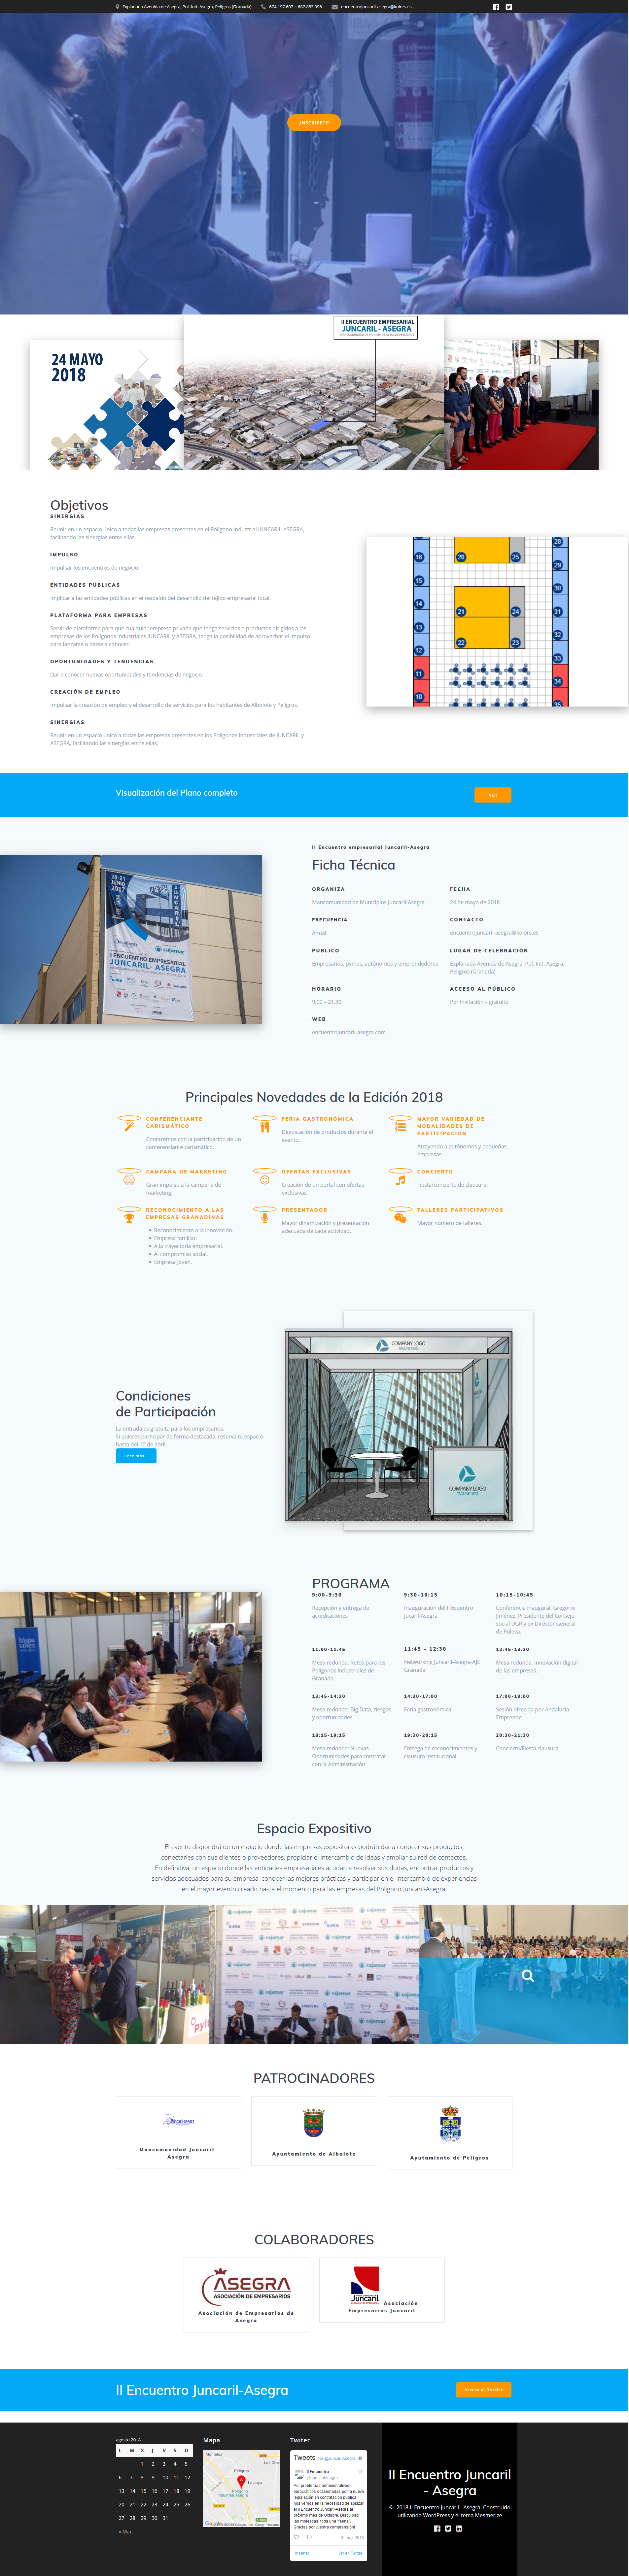
\includegraphics[scale=0.055]{image/juncaril.png}\\
			Página web - \href{http://encuentrojuncaril-asegra.com/}{Encuentro Juncaril Asegra}
		\end{center}
		
		\newpage
		
		\subsubsection{Deventos}
		
		\textbf{Descripción de la web}:
		
		Se podría dividir la construcción en dos partes para nuestro caso:\\
		
		\begin{itemize}
			\item \textbf{Diseño}: para el diseño de desarrollaron varios bocetos de la web, utilizando la herramienta pincel.\\
			
			Por otro lado todos los diagramas de diseño de la aplicación se descartaron por orden del jefe ya que tiene la falsa idea de no ser necesarios.\\
			
			\item \textbf{Desarrollo}: para el desarrollo de esta web se utiliza un wordpress desde cero siguiendo los siguientes pasos ya descritos anteriormente:
			\begin{enumerate}
				\item Instalar wordpress en Banahosting
				\item Instalar Un Certificado SLL Con Banahosting
			\end{enumerate}
			Ademas para la apariencia se utilizo la plantilla mesmerize PRO, que esta compuesta de diversos plugins que facilitan la organización y creación del espacio web junto con wordpress. No se puede mostrar el resultado final de esta web porque aun no esta terminada:\\ 
			
			\begin{center}
				\includegraphics[scale=0.2]{image/deventos.png}\\
				Página web - \href{https://www.deventos.es/}{Deventos}
			\end{center}
			
			\newpage
			
			Para el apartado de la tienda tanto de stand como de artículos se utilizo el plugins WooCommerce, el cual se modifico para que se dieran los siguientes resultados.
			
			\begin{center}
				\includegraphics[scale=0.35]{image/stand.png}\\
				Parte de Stand\\
				\includegraphics[scale=0.15]{image/mobi.png}\\
				Parte del mobiliario
			\end{center}
		\end{itemize}
		
		\newpage
		
		
		\section{Herramientas utilizadas para llevar a cabo el trabajo realizado}
		
		Podemos dividir las herramientas en dos grupo las usadas para el control del servidor y las usadas para diseño y desarrollo de la web.
		
		\subsection{Servidor}
		
		Las herramientas utilizadas para el control:
		
		\begin{itemize}
			\item \textbf{FileZilla} en sus versiones cliente o servidor, desarrollado para multiplataforma, de código abierto y software libre, licenciado bajo la Licencia Pública General de GNU. Soporta los protocolos FTP, SFTP y FTP sobre SSL/TLS (FTPS).
			 
			\item \textbf{cPanel de banahosting} (acrónimo de control Panel o ‘Panel de control’) es un panel de control para administrar servidores de alojamiento web que proveen herramientas de automatización y una interfaz gráfica basada en páginas web.
			
			Este software cuenta con un diseño en tres capas que entrega distintos atributos a administradores, revendedores de espacio y usuarios finales. Estos atributos permite controlar diversos aspectos de los servidores y servicios entregados a los clientes externos (usuarios de páginas web). Es software de tipo propietario y se ha desarrollado para ser compatible con la mayoría de las distribuciones de Linux que usen RPM como gestor de paquetes. 
		\end{itemize}
	
		\subsection{Página web}
		
		Las herramientas utilizadas para el diseño y desarrollo de la web son:
		
		\begin{itemize}
			\item \textbf{WordPress} es un sistema de gestión de contenidos o CMS (por sus siglas en inglés, Content Management System) enfocado a la creación de cualquier tipo de página web. Está desarrollado en el lenguaje PHP para entornos que ejecuten MySQL y Apache, bajo licencia GPL y es software libre. Actualizado con los siguientes plugins:
			\begin{itemize}
				\item \textbf{Akismet}: Servicio anti-spam, funciona muy bien. Es gratis para sitios personales y de pago para sitios  comerciales (que generen ingresos). 
				\item \textbf{BackWPup}: Fantástico plugin gratuito para la creación automáticas de copias de seguridad, nos gusta por su flexibilidad de configuración, su fiabilidad y su integración con servicios en la nube (en nuestro caso, las copias se guardan en nuestra cuenta de SugarSync).
				\item \textbf{Google Analytics for WordPress}: Este plugin inserta automáticamente el código de tracking que Google Analytics necesita para poder recopilar sus estadísticas del blog.
				\item \textbf{WooCommerce}: Este plugin es simplemente la caña si quieres montarte una pequeña tienda de comercio electrónico en tu blog. Tienes todo lo importante: catálogo de productos, gestión de las ventas, medios de pago… En fin, muy completo y gratis en su versión básica.
			\end{itemize} 
		\end{itemize}
		
		
		
		\newpage
		
		\section{Asignaturas de la titulación que hayan resultado útiles para llevar a cabo el trabajo realizado}
		Aunque cualquier asignatura a lo largo de la carrera es ilustrativa a la hora de pensar como un ingeniero en formación, algunas de las asignaturas que fueron más útiles durante el trabajo son las siguientes:
		
		\begin{itemize}
			\item \textbf{Página web:} resultaron de utilidad \textit{Tecnologías Web (TW)} y \textit{Programación Web (PW)}. Estas dos asignaturas de diseño web que cursé y curso, enfoca todos los fundamentos de las páginas web.
			\item \textbf{Servidor web:} resultaron de utilidad \textit{Servidores Web de Altas Prestaciones (SWAP)} y \textit{Ingeniería de Servidores (ISE)}. Estas dos asignaturas de manejo de servidores me fueron de gran ayuda a la hora de configurar el servidor.
		\end{itemize}
		
		\newpage
		
	\part{Bibliografía utilizada}
		Entre la bibliografía utilizada de carácter general, se encuentra la siguiente lista:
		
		\begin{itemize}
			\item Manual de Cascading StyleSheet - \href{https://www.w3schools.com/css/default.asp}{w3schools.com CSS Tutorial}
			\item W3.CSS Faster and better fully responsive CSS - \href{https://www.w3schools.com/w3css/default.asp}{w3schools.com W3.CSS}
			\item YouTube
			\item Taringa
			
		\end{itemize}
		
		Por otro lado, hice buen provecho de foros de gran volumen como Stack Overflow, dado que muchos usuarios realizan preguntas muy específicas al toparse con un problema, y gente las resuelve sin llegar a redactar ningún artículo extenso al respecto.
		
		\newpage
		
	\part{Valoración personal del trabajo realizado}
	
		Personalmente, me siento muy satisfecho con el trabajo realizado. Para empezar, las condiciones que me brindó la empresa fueron sensacionales, empezando por la flexibilidad de horarios y continuando con la importancia de la palabra de cada empleado; dándome ánimos a dar un paso adelante, a pensar en el futuro del proyecto sintiéndome parte de él y a tomar decisiones responsables que lo acompañasen.\\
		
		Además, estos meses de trabajo con la empresa me han servido para aprender a manejar un servidor web y la utilización de aplicaciones web. Por si fuera poco, al enfrentarme yo y mi compañera en practicas solos a esta tarea, nos proporciono libertad a la hora de idear y estudiar soluciones y/o posibles propuestas. Esto no quiere decir que estuviera solo, ya que antes de proceder tras tomar una decisión la comentaba con el resto del equipo, ya que \textit{cuatro ojos ven más que dos} y cualquiera puede estar equivocado aunque no lo piense.\\
		
		
	
	\newpage
	
	\part{Conclusiones}
	
		Como conclusión quisiera destacar, que el período de prácticas de empresa me parecen una experiencia prácticamente obligada para cualquier estudiante del grado, tanto de Ingeniería Informática como de cualquier carrera técnica, y algo que ya he recomendado y que seguiré recomendando a cualquier estudiante que conozca. Independientemente de si al finalizar esta temporada se produce una contratación por parte de la empresa o no, el hecho de enfrentarse a un proyecto real genera mucha madurez tanto personal como profesional. Además de la ayuda económica que suponen este y cualquier trabajo, \textbf{la formación vale mucho dinero}; y como estudiante es una etapa indispensable en la que la persona aprende a organizarse en su vida personal para compaginar estudios y empleo, además de entrenarse con la estimación de los intervalos de tiempo necesarios para el desempeño de futuros proyectos.\\
		
		Para terminar, agradezco la oportunidad brindada para seguir en la empresa y formar parte de un proyecto tan interesante sin siquiera haber finalizado el grado.
	
		\newpage

\end{document}
